\section{Results}

\subsection{From sparse equations to a dielectric}

The compiler takes a nonsingular rational system $Mx=b$ with $m$ nonzero
matrix entries and a requested accuracy $\eta$, measured as the relative
residual $\norm{Mx-b}_2\le\eta\norm b_2$. Two numerical conditions define the
class of inputs: the condition number $\kappa_2(M)$ grows at most as a fixed
power of $m$, and $\eta$ decreases at most as a fixed inverse power of $m$.
Each coefficient has $O(\log m)$ bits. These conditions fix the accuracy
regime, while the pattern of couplings between unknowns is unrestricted.

The translation proceeds in three stages (\cref{fig:concept}). First, the
system is rewritten as a \emph{logical network}, i.e., a sparse symmetric
system in which every site couples to at most three neighbors with a coupling
from a small fixed set of values. Auxiliary sites copy variables, add
contributions and mediate signs, so that a row or column of $M$ with many
nonzero entries is spread over many sites of low degree. The network
determines the original solution through a fixed set of its sites, and a small
residual in the network implies a small residual in $Mx=b$. Second, the network
is routed through a three-dimensional cubic grid, with every edge replaced by a
path of nearest-neighbor steps and with enough space between paths that they
do not interact. Third, every site of the routed network becomes a localized
electromagnetic mode in a dielectric background, and the physical couplings between
neighboring modes reproduce the couplings of the network.

The volume is set by the routing stage. The logical network has
$O(m\log m)$ sites, and it can be routed in a cubic box whose sides grow as
$O(\sqrt{m\log m})$, which gives a volume of $\Ot(m^{3/2})$. This is the same exponent that Kolmogorov and
Barzdin found for embedding general networks with wires of finite thickness in
three dimensions, where it is optimal for networks with good expansion
properties~\citep{KolmogorovBarzdin1967,GromovGuth2012}. The separation between
modes and the buffer to the boundary add only logarithmic factors.

\begin{figure}[tbp]
\centering
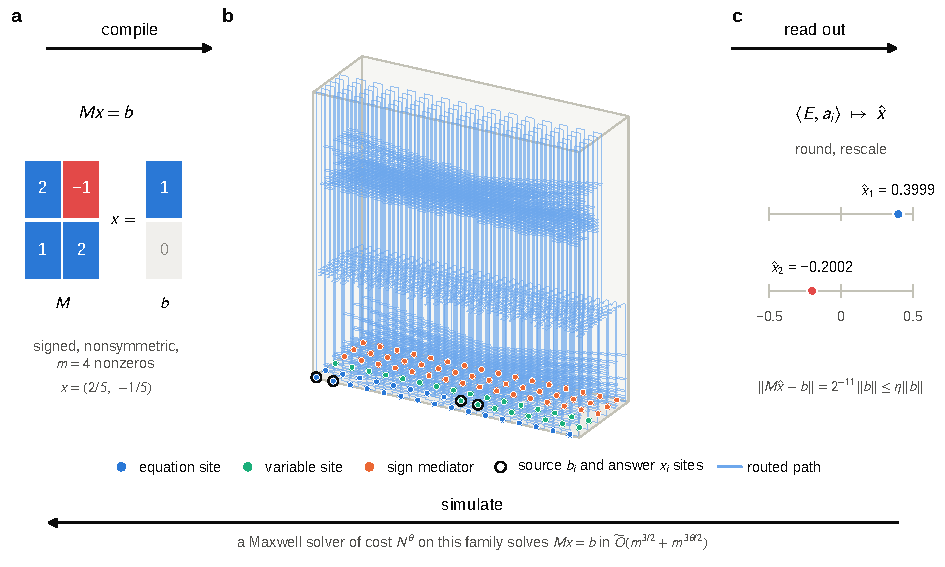
\includegraphics[width=\linewidth]{figures/fig1_concept.pdf}
\caption{\textbf{A sparse linear system and a dielectric cavity encode each other.}
\textbf{a}, The input is a sparse system $Mx=b$ with $m$ signed rational coefficients; shown is the
$2\times2$ example $M=\bigl(\begin{smallmatrix}2&-1\\1&2\end{smallmatrix}\bigr)$, $b=(1,0)$, whose
solution is $x=(2/5,\,-1/5)$. Blue and red cells are positive and negative entries.
\textbf{b}, The compiler expresses the equations through a local network of 96 sites (equation sites,
variable sites and sign mediators, each connected to at most three others) and routes its 96
connections as paths through a $505\times169\times3105$ integer grid. The drawing is the network the
compiler produced for the example in a, with the routing axis compressed sixfold for display; the paths
are long because the compiler equalizes their lengths. Each site becomes a broad, weak defect in the
periodic dielectric that fills the box, each path becomes a chain of such defects, and the walls are
perfect conductors. Ringed sites carry the source $b$ and the answer $x$.
\textbf{c}, A finite list of field moments $\langle E,a_i\rangle$ at the answer sites, rounded and
rescaled, returns $\hat x$. For the example, exact arithmetic on the compiled network gives
$\hat x=(819/2048,\,-205/1024)$ with relative residual $2^{-11}$, within the requested tolerance
$\eta=1/4$. Read from left to right (compile, read out), the cavity is an optical computer for $Mx=b$;
read from right to left (simulate), a Maxwell solver that handles this family of cavities in time
$N^{\theta}$, where $N$ counts grid cells, is a sparse linear solver of cost
$\widetilde O(m^{3/2}+m^{3\theta/2})$.}
\label{fig:concept}
\end{figure}

The output of the compiler is a complete electromagnetic problem. For the
continuum construction, it consists of the permittivity $\varepsilon(r)$ in a
rectangular box $\Omega$ with perfectly electrically conducting (PEC) walls, a
square-integrable current source $f$ and a list of weighting functions
$a_i$, such that the time-harmonic electric field $E$ solves
\begin{equation}
 \nabla\times\nabla\times E-\varepsilon E=f
 \quad\text{in }\Omega,\qquad
 \hat n\times E=0\quad\text{on }\partial\Omega,
 \label{eq:maxwell}
\end{equation}
in units in which the frequency and the permeability are one. The answer is
read from the moments $\ip{E}{a_i}$, i.e., from weighted volume integrals of
the field. The permittivity is real, scalar and bounded, $1\le\varepsilon\le25$;
the continuum construction in fact uses only values between 6 and 10. The
discrete construction outputs the corresponding Yee system with one
permittivity value per grid cell, at a fixed resolution of ten cells per
shortest wavelength in the material, and reads the answer from prescribed
field coordinates. Both constructions use the same logical network and routing
and differ in how the network is realized physically. The guarantees they
share are summarized in \cref{tab:guarantees}.

\begin{table}[tbp]
\centering
\caption{\textbf{Guarantees of the compiler.} The left column lists the
quantities that determine whether the translation between a sparse system
$Mx=b$ with $m$ nonzero coefficients and an electromagnetic problem is
efficient; the right column gives the bound proved for each. Size, encoding
and decoding bounds hold for every run of the randomized encoder, and count
the complete box including empty background, routing space and the buffer to
the walls. Conditioning and recovery hold together with probability at least
$1-3/(64m)$ for $m\ge2$: on this event, every field whose relative Maxwell
residual is at most $\delta$ decodes to an approximate solution with relative
residual at most $\eta$. The bounds apply to both the continuum and the Yee
construction. Constants and powers of logarithms depend only on the fixed
input class and are not optimized.}
\label{tab:guarantees}
\small
\begin{tabularx}{\linewidth}{@{}p{0.32\linewidth}X@{}}
\toprule
Quantity & Guarantee \\
\midrule
Size of the structure & $\Ot(m^{3/2})$, counting the whole box: background, routing space and buffer \\
Encoding and decoding & $\Ot(m^{3/2})$ bit operations \\
Coefficients and readout & $O(\log m)$ bits each \\
Permittivity & Real, scalar, $1\le\varepsilon\le25$; PEC only at the outer walls \\
Conditioning & Polynomial in $m$ for the full electromagnetic operator \\
Field accuracy required & Relative residual $\delta\ge m^{-c_\delta}$ for a fixed $c_\delta$ \\
Recovery & Every field meeting this residual decodes to an answer with relative residual $\le\eta$ \\
\bottomrule
\end{tabularx}
\end{table}

\subsection{Defect modes as unknowns}

The central difficulty is the third stage. A network of mode amplitudes is
useful only if the actual Maxwell field -- including all components that are
not part of the network -- reproduces its equations to the required accuracy.
The required couplings shrink as the problem grows, since the encoded errors
must fall below an inverse polynomial of $m$, and the unwanted couplings must
remain smaller still after summation over all $\Ot(m^{3/2})$ sites.

The background is a weakly modulated periodic dielectric,
\begin{equation}
 \varepsilon_{\rm per}(r)=7+\varrho
 \bigl[\cos(\pi r_1)+2\cos(\pi r_2)+4\cos(\pi r_3)\bigr],
 \label{eq:background}
\end{equation}
with $\varrho=2^{-100}$ and period two in each direction. In a
homogeneous medium, the eight plane waves with wavevectors
$(\pm\pi/2,\pm\pi/2,\pm\pi/2)$ are degenerate at the corner
$k_*=(\pi/2,\pi/2,\pi/2)$ of the Brillouin zone, which gives a cluster of
sixteen states once both polarizations are counted. The modulation, with its
three distinct amplitudes, splits this cluster, and we prove that one of the
resulting branches of the operator $\nabla\times\nabla\times-\varepsilon_{\rm per}$
has an isolated, nondegenerate local minimum at $k_*$, i.e., near $k_*$ the
branch rises quadratically in every direction (\cref{fig:mechanism}a,b). The
splitting of the cluster is verified in exact rational arithmetic, and
analytic estimates over all other Fourier components extend the statement to
the continuum.

A band minimum acts locally like a band edge. Slightly raising the
permittivity over a broad region binds a mode just below the minimum,
in the same way as a defect in a photonic crystal binds a mode inside a band
gap~\citep{figotinklein1997,figotinklein1998,Joannopoulos2008}. The mode is
the envelope of the Bloch wave at $k_*$ and decays exponentially away from
the defect. Two such modes at distance $d$ couple through their overlapping
tails, which gives a tight-binding description of the defect lattice in the
spirit of coupled-resonator waveguides and Wannier-function models of
photonic-crystal circuits~\citep{Yariv1999,Busch2003}. We prove matching
bounds on this coupling. Along the three routing directions, the useful
nearest-neighbor coupling is at least of order $8^{-d}$, while the coupling
between defects that are $\nu$ lattice steps apart is at most of order
$3^{-d\norm{\nu}_1}$. The routing places the sites such that
only sites connected in the network are lattice neighbors, so every unwanted
coupling spans at least two lattice steps. Since $(1/3)^2<1/8$, each of these
couplings is smaller than the useful one by a factor that grows exponentially
in $d$ (\cref{fig:mechanism}c). A separation $d$ that grows
only logarithmically in $m$ therefore suppresses the sum of all unwanted
couplings below any required inverse polynomial.

Signs and asymmetry are produced by elimination. A dielectric is reciprocal,
and the coupling between two identical modes has a fixed sign, whereas $M$ is
an arbitrary signed, nonsymmetric matrix. The logical network solves this at
the algebraic level: the original system is embedded in a larger symmetric
system, and auxiliary \emph{mediator} sites, detuned by small changes of their
local permittivity, produce effective couplings of either sign once their
amplitudes are eliminated, i.e., through a Schur complement (\cref{fig:mechanism}d). The physical
construction only has to realize nearest-neighbor couplings of one sign and
tunable on-site energies, which is exactly what the defect lattice provides.

\begin{figure}[tbp]
\centering
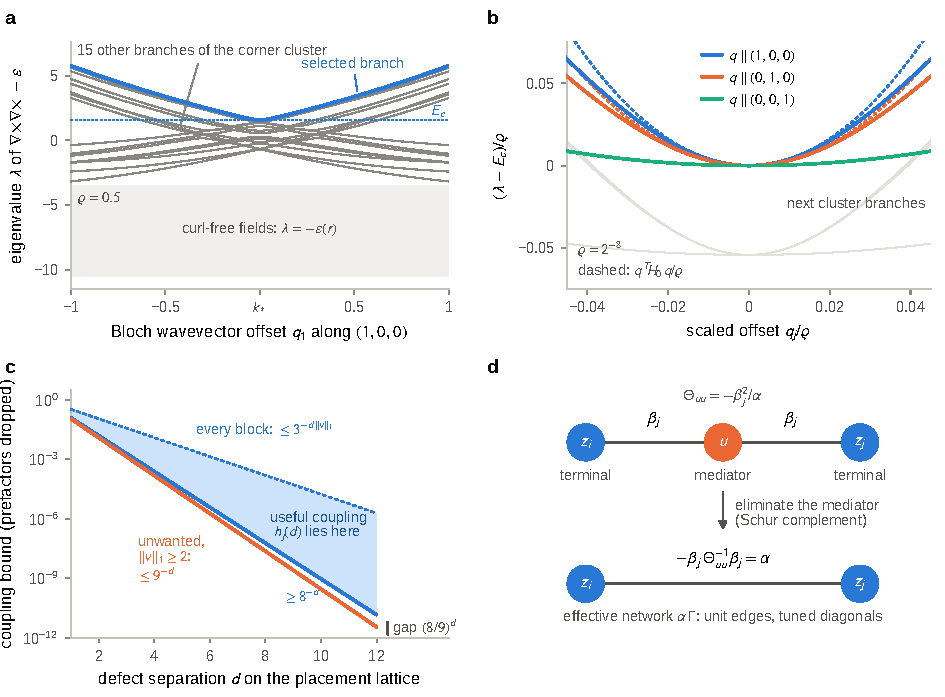
\includegraphics[width=\linewidth]{figures/fig2_mechanism.pdf}
\caption{\textbf{Broad defects in a weakly modulated dielectric interact like a network.}
\textbf{a}, Bloch spectrum of $\nabla\times\nabla\times-\varepsilon(r)$ for the periodic background
$\varepsilon=7+\varrho\,[\cos\pi r_1+2\cos\pi r_2+4\cos\pi r_3]$ along the line $k=k_*+q_1(1,0,0)$
through $k_*=(\pi/2,\pi/2,\pi/2)$, computed with a vector plane-wave expansion (1029 plane-wave
components; eigenvalues converged to $10^{-7}$). The modulation is exaggerated to $\varrho=0.5$ for
visibility; the construction uses $\varrho=2^{-100}$. At $k_*$ eight plane waves of the unmodulated
medium are degenerate, forming a cluster of sixteen transverse branches that the modulation splits.
The selected branch (blue) is the highest of them and has an isolated local minimum $E_c$ at $k_*$.
Curl-free fields contribute the band $\lambda=-\varepsilon(r)$ (gray), and the other cluster branches
cross $E_c$ away from $k_*$: there is no complete gap, and the proof bounds leakage into these states
instead of assuming its absence.
\textbf{b}, The selected branch near $k_*$ along the three axes, computed at $\varrho=2^{-8}$ and drawn
in scaled variables, in which the curves no longer change as $\varrho\to0$. Dashed: the quadratic form
$q^{T}\!H_0\,q/\varrho$ with the exact leading-order Hessian of the proof,
$H_0=\pi^2\,\mathrm{diag}(4.12,\,3.26,\,0.44)$; the next branches of the cluster (light gray) stay
$0.054\,\varrho$ below the minimum.
\textbf{c}, Proven decay rates of the interaction between two defects $d$ placement-lattice steps
apart, with constant prefactors dropped: the useful nearest-neighbor coupling $h_j(d)$ is at least
$8^{-d}$ and, like every interaction block, at most $3^{-d}$, whereas every block between defects
that are not nearest neighbors is at most $9^{-d}$. The gap between the two rates is $(8/9)^{d}$:
because $9>8$, the summed unwanted couplings fall below the useful ones once $d=O(\log m)$.
\textbf{d}, A sign mediator $u$ between two terminals $z_i$, $z_j$ with couplings $\beta_j$ and tuned
self-term $\Theta_{uu}=-\beta_j^2/\alpha$; eliminating it leaves the effective coupling $\alpha$, so the
defect amplitudes obey $\alpha\Gamma z=\alpha g$ for the compiled network matrix $\Gamma$, which has
unit edges and tuned diagonals.}
\label{fig:mechanism}
\end{figure}

A local band minimum is not a complete band gap. Other Bloch waves propagate
at the operating frequency elsewhere in momentum space, and a defect mode can
leak into them. The defects are therefore made broad and smooth, with radius
$L$ and permittivity change of order $L^{-2}$, so that their momentum content
is concentrated near $k_*$. The leakage then decays as $e^{-cL^{1/3}}$, and a
defect radius growing as a power of $\log m$ suffices. The momentum window
used to separate the useful channel from the remaining waves is a tool of the
analysis, not a feature of the structure, and all leakage enters the residual
of the actual Maxwell equation, together with the errors from the finite
boundary and the finite description of the material.

The last step controls the response of the cavity as a whole. A lossless
cavity has resonances, and near a resonance a small residual can produce a
large field error. A small uniform shift of the permittivity, drawn at random
after all other parameters are fixed, avoids every resonance by a margin that
is polynomial in $m$ with high probability. On this event, the inverse of the
full Maxwell operator is bounded polynomially in $m$, which is what allows the
leakage to be tolerated instead of eliminated.

\subsection{Approximate fields give approximate answers}

The recovery guarantee is stated in terms of quantities that a solver can
check. Writing $A$ for the Maxwell operator of \cref{eq:maxwell}, the compiler
outputs a field tolerance $\delta$ such that
\begin{equation}
 \norm{AE-f}\le\delta\norm f
 \quad\Longrightarrow\quad
 \norm{Mx-b}_2\le\eta\norm b_2,
 \label{eq:recovery}
\end{equation}
where $x$ is decoded from the moments of $E$. The implication holds for every
field $E$ that meets the residual bound, irrespective of how it was obtained,
including complex fields of any polarization. The tolerance $\delta$ decreases
only polynomially with $m$, and the decoder needs each moment only to
$O(\log m)$ bits of precision. Since the bounded inverse makes the field
error at most polynomially larger than its residual, every admissible field
lies close to a reference field constructed in the proof, and the moments of
the reference field encode a solution of the logical network to within the
budget of \cref{eq:recovery}.

The material, source and weighting functions are themselves outputs of finite
size. The permittivity consists of the fixed trigonometric background,
dyadic shifts and polynomial profiles on balls whose radii and spacing grow
with $m$; there are no shrinking features, thin gaps or interior conductors.
Computing these descriptions does not require solving the assembled Maxwell
problem. Instead, the encoder calibrates the defect parameters once, from
finite algebra at $k_*$ and controlled Fourier tails, and every approximation
error is propagated to the final answer.

\subsection{Numerical illustrations}

Two small numerical realizations illustrate complementary parts of the encoding
(\cref{fig:numerical}). First, we calibrate six smooth dielectric defects in a
three-dimensional periodic cavity to a prescribed signed $3\times3$ matrix
$\Gamma$. Three defects carry the sources and readout functions, while three
auxiliary defects adjust the cavity response. The material remains scalar and
positive, with $4.77<\varepsilon<21.24$. Once calibrated, the structure,
source profiles and decoder are fixed, and changing the source amplitudes
changes the right-hand side. A full-vector Maxwell solve on the finer grid
gives $\norm{\Gamma X-I}_2=7.88\times10^{-4}$, where $X$ is the decoded
response to all basis inputs; this bounds the relative equation error for
every right-hand side.

Second, we assemble several systems from one locally calibrated component in
a rectangular PEC waveguide. Its transverse symmetry gives a single invariant
channel, with confinement supplied by waveguide cutoff. An isolated well
determines a resonance parameter $\mu$, and its evanescent tail determines
the coupling $t$ between neighboring wells. For a chain with off-diagonal
entries $-1$, the material strengths follow directly from
$v_i=(\mu+t\Gamma_{ii})^{-1}$. This rule transfers from three to four sites
without changing the common strength, and a detuned auxiliary well produces
a positive effective coupling by elimination. Five prescribed targets,
including an indefinite chain, have equation errors below $0.55\%$ on both
finer full-vector grids, with the assembled responses used only for
verification. The component calibration, refinement tests and material-precision
study are given in Section~\ref{n:sec:numerical} of the \SI.

\begin{figure}[tbp]
\centering
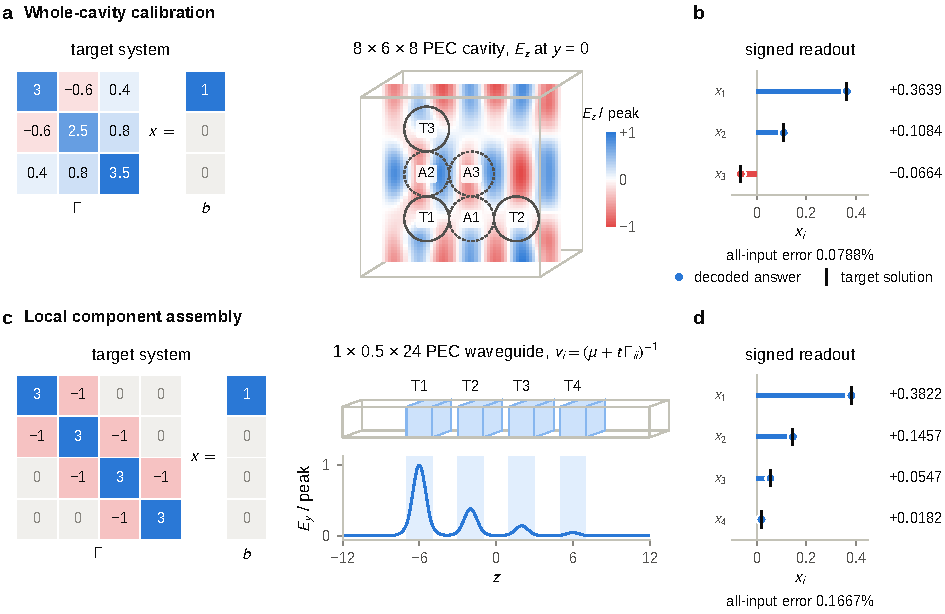
\includegraphics[width=\linewidth]{figures/fig_numerical.pdf}
\caption{\textbf{Calibrated cavities and reusable components give two numerical realizations.}
\textbf{a}, A prescribed signed matrix is encoded by six smooth spherical
dielectric defects in an $8\times6\times8$ PEC cavity. The plotted section is
the signed electric-field phasor $E_z$ at $y=0$ for $b=(1,0,0)$, normalized by
its peak absolute value in the section. Solid circles mark the support of the
three terminal defects T1--T3; dashed circles mark the auxiliary defects A1--A3.
The full three-dimensional material strengths were calibrated against the
cavity response and held fixed during refinement.
\textbf{b}, Signed volume moments give the decoded answer (circles), compared
with the target solution (black ticks). The reported error $\norm{\Gamma X-I}_2$
covers all inputs; the displayed field was computed at $h=1/7$.
\textbf{c}, Four translated copies of one dielectric well realize a chain
using the local rule $v_i=(\mu+t\Gamma_{ii})^{-1}$. Blue regions mark the
supports of smooth wells spanning the waveguide cross-section; the transverse
dimensions are enlarged. The curve is the computed $E_y$ along the centerline
for $b=(1,0,0,0)$ at $h=1/22$, normalized by its peak absolute value.
\textbf{d}, The same local source and readout construction recovers the
four-component answer, with all-input error $0.1667\%$.}
\label{fig:numerical}
\end{figure}

\subsection{Consequences for electromagnetic solvers}

The compiler is an algorithm in its own right: encode $Mx=b$, call an
electromagnetic solver, and decode its output. Suppose a solver handles the
constructed family uniformly, in time $O(N^\theta)$ for a structure of size $N$,
with only logarithmic dependence on the condition number and on the requested
accuracy, and returns the required moments. Substituting $N=\Ot(m^{3/2})$ gives
\begin{equation}
 T_{\rm sparse}(m)=\Ot\!\left(m^{3/2}+m^{3\theta/2}\right),
 \label{eq:transfer}
\end{equation}
where the first term accounts for encoding and decoding, and the second for
the electromagnetic solve (\cref{fig:consequence}). This implication is
unconditional. For polynomially conditioned systems with $O(n)$ nonzero
entries, the best known algorithm runs in $\Ot(n^2)$ bit
operations~\citep{kelner2026}, improving on earlier algorithms that beat matrix
multiplication~\citep{pengvempala2021,nie2022}. A uniform Maxwell solver with
$\theta<4/3$ would therefore solve sparse linear systems faster than any known
method. For comparison, nested dissection solves three-dimensional grid
problems directly in time $O(N^2)$, i.e., $\theta=2$~\citep{George1973,LiptonRoseTarjan1979}.

A lower bound on Maxwell solvers requires, in addition, a hypothesis about the
difficulty of sparse linear algebra. Assuming that no randomized algorithm
solves the input class in time $\Ot(m^{\gamma'})$ for any $\gamma'<\gamma$, for some
$\gamma>3/2$ -- a randomized version of the hypothesis used for
structured linear systems and packing linear
programs~\citep{kyngzhang2017,kyng2020} -- \cref{eq:transfer} excludes uniform
Maxwell solvers with $\theta<2\gamma/3$. Known algorithms restrict the
hypothesis to $\gamma\le\min\{2,1+c_\kappa\}$, where $m^{c_\kappa}$ bounds the condition
number, so the strongest consequence of this kind excludes $\theta<4/3$ --
the same threshold below which a Maxwell solver would improve on the best known
sparse algorithms. The
statement concerns solvers that work on the whole constructed family with the
stated dependence on conditioning and accuracy; restricted geometries,
well-conditioned problems or less accurate outputs can admit faster
algorithms.

\begin{figure}[tbp]
\centering
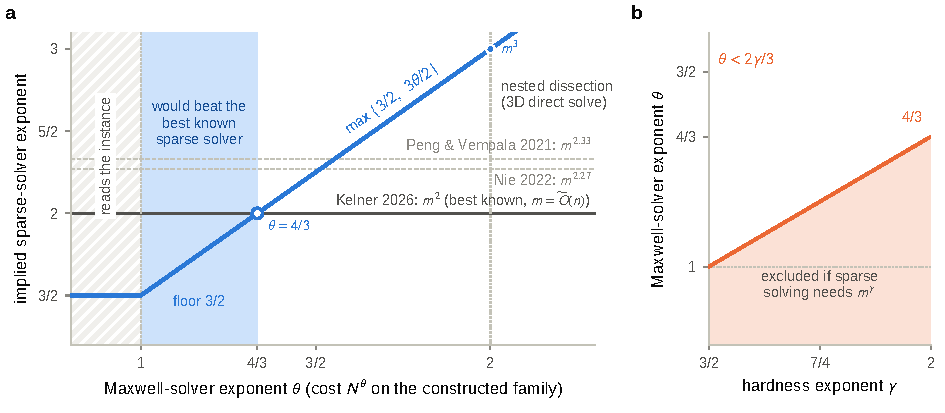
\includegraphics[width=\linewidth]{figures/fig3_consequence.pdf}
\caption{\textbf{What a fast Maxwell solver would mean for sparse linear algebra.}
\textbf{a}, If a solver handles every cavity of the constructed family in time $N^{\theta}$ up to
logarithmic factors, where $N$ counts grid cells and description length, then encoding, solving and
decoding solve every polynomially conditioned sparse system with $m$ nonzeros in time
$m^{\max\{3/2,\,3\theta/2\}}$ up to logarithmic factors (blue; the floor $3/2$ is the cost of encoding
and decoding). Horizontal lines are known bit-complexity upper bounds for the same problem class
($m=\widetilde O(n)$ nonzeros, polynomial condition number): the
$\widetilde O(mn\log(\kappa/\eta))$ algorithm of Kelner~\cite{kelner2026} gives $m^{2}$ and
supersedes the $m^{2.33}$ of Peng and Vempala~\cite{pengvempala2021,PengVempala2025} and the
$m^{2.27}$ of Nie~\cite{nie2022} (both stated with the bound $2.3729$ on the matrix-multiplication exponent
used in those papers). Vertical
lines mark $\theta=1$, below which a solver can not read its input, and $\theta=2$, the cost of a
nested-dissection direct solve on a three-dimensional grid~\cite{George1973,LiptonRoseTarjan1979}. A
uniform solver with $1\le\theta<4/3$ (shaded) would improve the best known sparse-solver exponent.
The statement concerns worst-case solvers on this family of cavities.
\textbf{b}, Conversely, if solving sparse systems requires time $m^{\gamma}$ for some
$\gamma\in(3/2,2]$, the range compatible with the $m^{2}$ upper bounds (conjugate gradients in exact
arithmetic in the real-arithmetic model of the hypothesis; Kelner's algorithm in the bit model), no
uniform Maxwell solver for the family can have $\theta<2\gamma/3$ (shaded).}
\label{fig:consequence}
\end{figure}
